\documentclass[tikz,convert={outfile=\jobname.svg}]{standalone}
\usepackage[utf8]{inputenc}
\usepackage{tikz}
    \begin{tikzpicture}		
  		\matrix
  		{
  			\node [text width=10cm]{\emph{Self-tapping screws} are tapered and have a coarse thread. They are used in soft materials where an undersized, plain pilot hole has been drilled. A 2.9x9mm self-tapping screw has a nominal thread width of 2.9mm and a thread length of 9mm.};&
  			\node {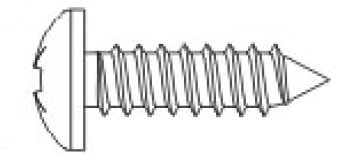
\includegraphics[width=2cm]{graphics/self-tap}};\\
  			
  			\node [text width=10cm]{\emph{Machine screws} are straight and have a fine thread. They are fastened with nuts or where a threaded hole has been cut. An M3x10mm machine screw has a thread of nominal 3mm diameter and a thread length of 10mm.};&
  			\node {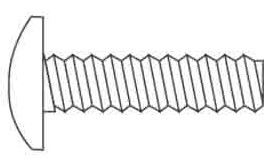
\includegraphics[width=2cm]{graphics/screw}};\\
  		};
  	\end{tikzpicture}
\end{document}
